\documentclass[dvisvgm,multi=true]{standalone}
\usepackage{mathmlcoresvg}
\begin{document}
%<figcaption><span>Figure 17: </span>Box model for the <code>horizontalstrike</code>
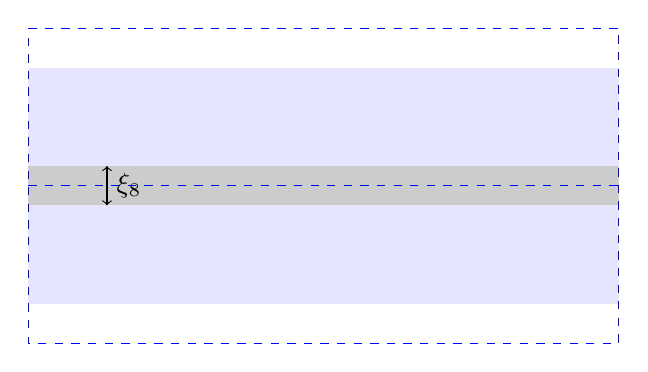
\begin{tikzpicture}[yscale=-1]

  \fill[blue!10] (0,-1.5) -- (7.5,-1.5) -- (7.5,1.5) -- (0,1.5) -- cycle;

  \MathMLBox{0}{0}{1.5}{1}{red};

  \fill[black!20] (0,-.25) -- (7.5,-.25) -- (7.5,.25) -- (0,.25) -- cycle;

  \draw[dashed,blue](0,-2) -- (7.5,-2) -- (7.5,2) -- (0,2) -- cycle
  (0,0) -- (7.5,0);

  \draw[<->] (1,-.25) -- (1,0) node[right]{$\xi_8$} -- (1,.25);
\end{tikzpicture}

\end{document}
